\documentclass[a4paper]{article}
\usepackage[warn]{mathtext}
\usepackage[utf8]{inputenc}
\usepackage[T2A]{fontenc}
\usepackage[english,russian]{babel}
\usepackage{multicol}
\usepackage{fancyhdr}
\usepackage{graphicx}
\usepackage{microtype}
\usepackage{wrapfig}
\usepackage{amsmath}
\usepackage{floatflt}
\usepackage{geometry} \geometry{verbose,a4paper,tmargin=2cm,bmargin=2cm,lmargin=1.5cm,rmargin=1.5cm}
\usepackage{float}
\usepackage{amssymb}
\usepackage{caption}
\usepackage{epsfig}
\usepackage{newunicodechar}

\begin{document}

\graphicspath{ {pictures/} }
\begin{center}
    {\scshape\Large Лабораторная работа по твердотельной электронике} \par

    \

    {\huge\bfseries № 17: Исследование рекомбинации и генерации в полупроводниках} \par 

    \

    {\large Яромир Водзяновский Б04-852}
\end{center}

\

\

\begin{figure}[H]
    \begin{center}
        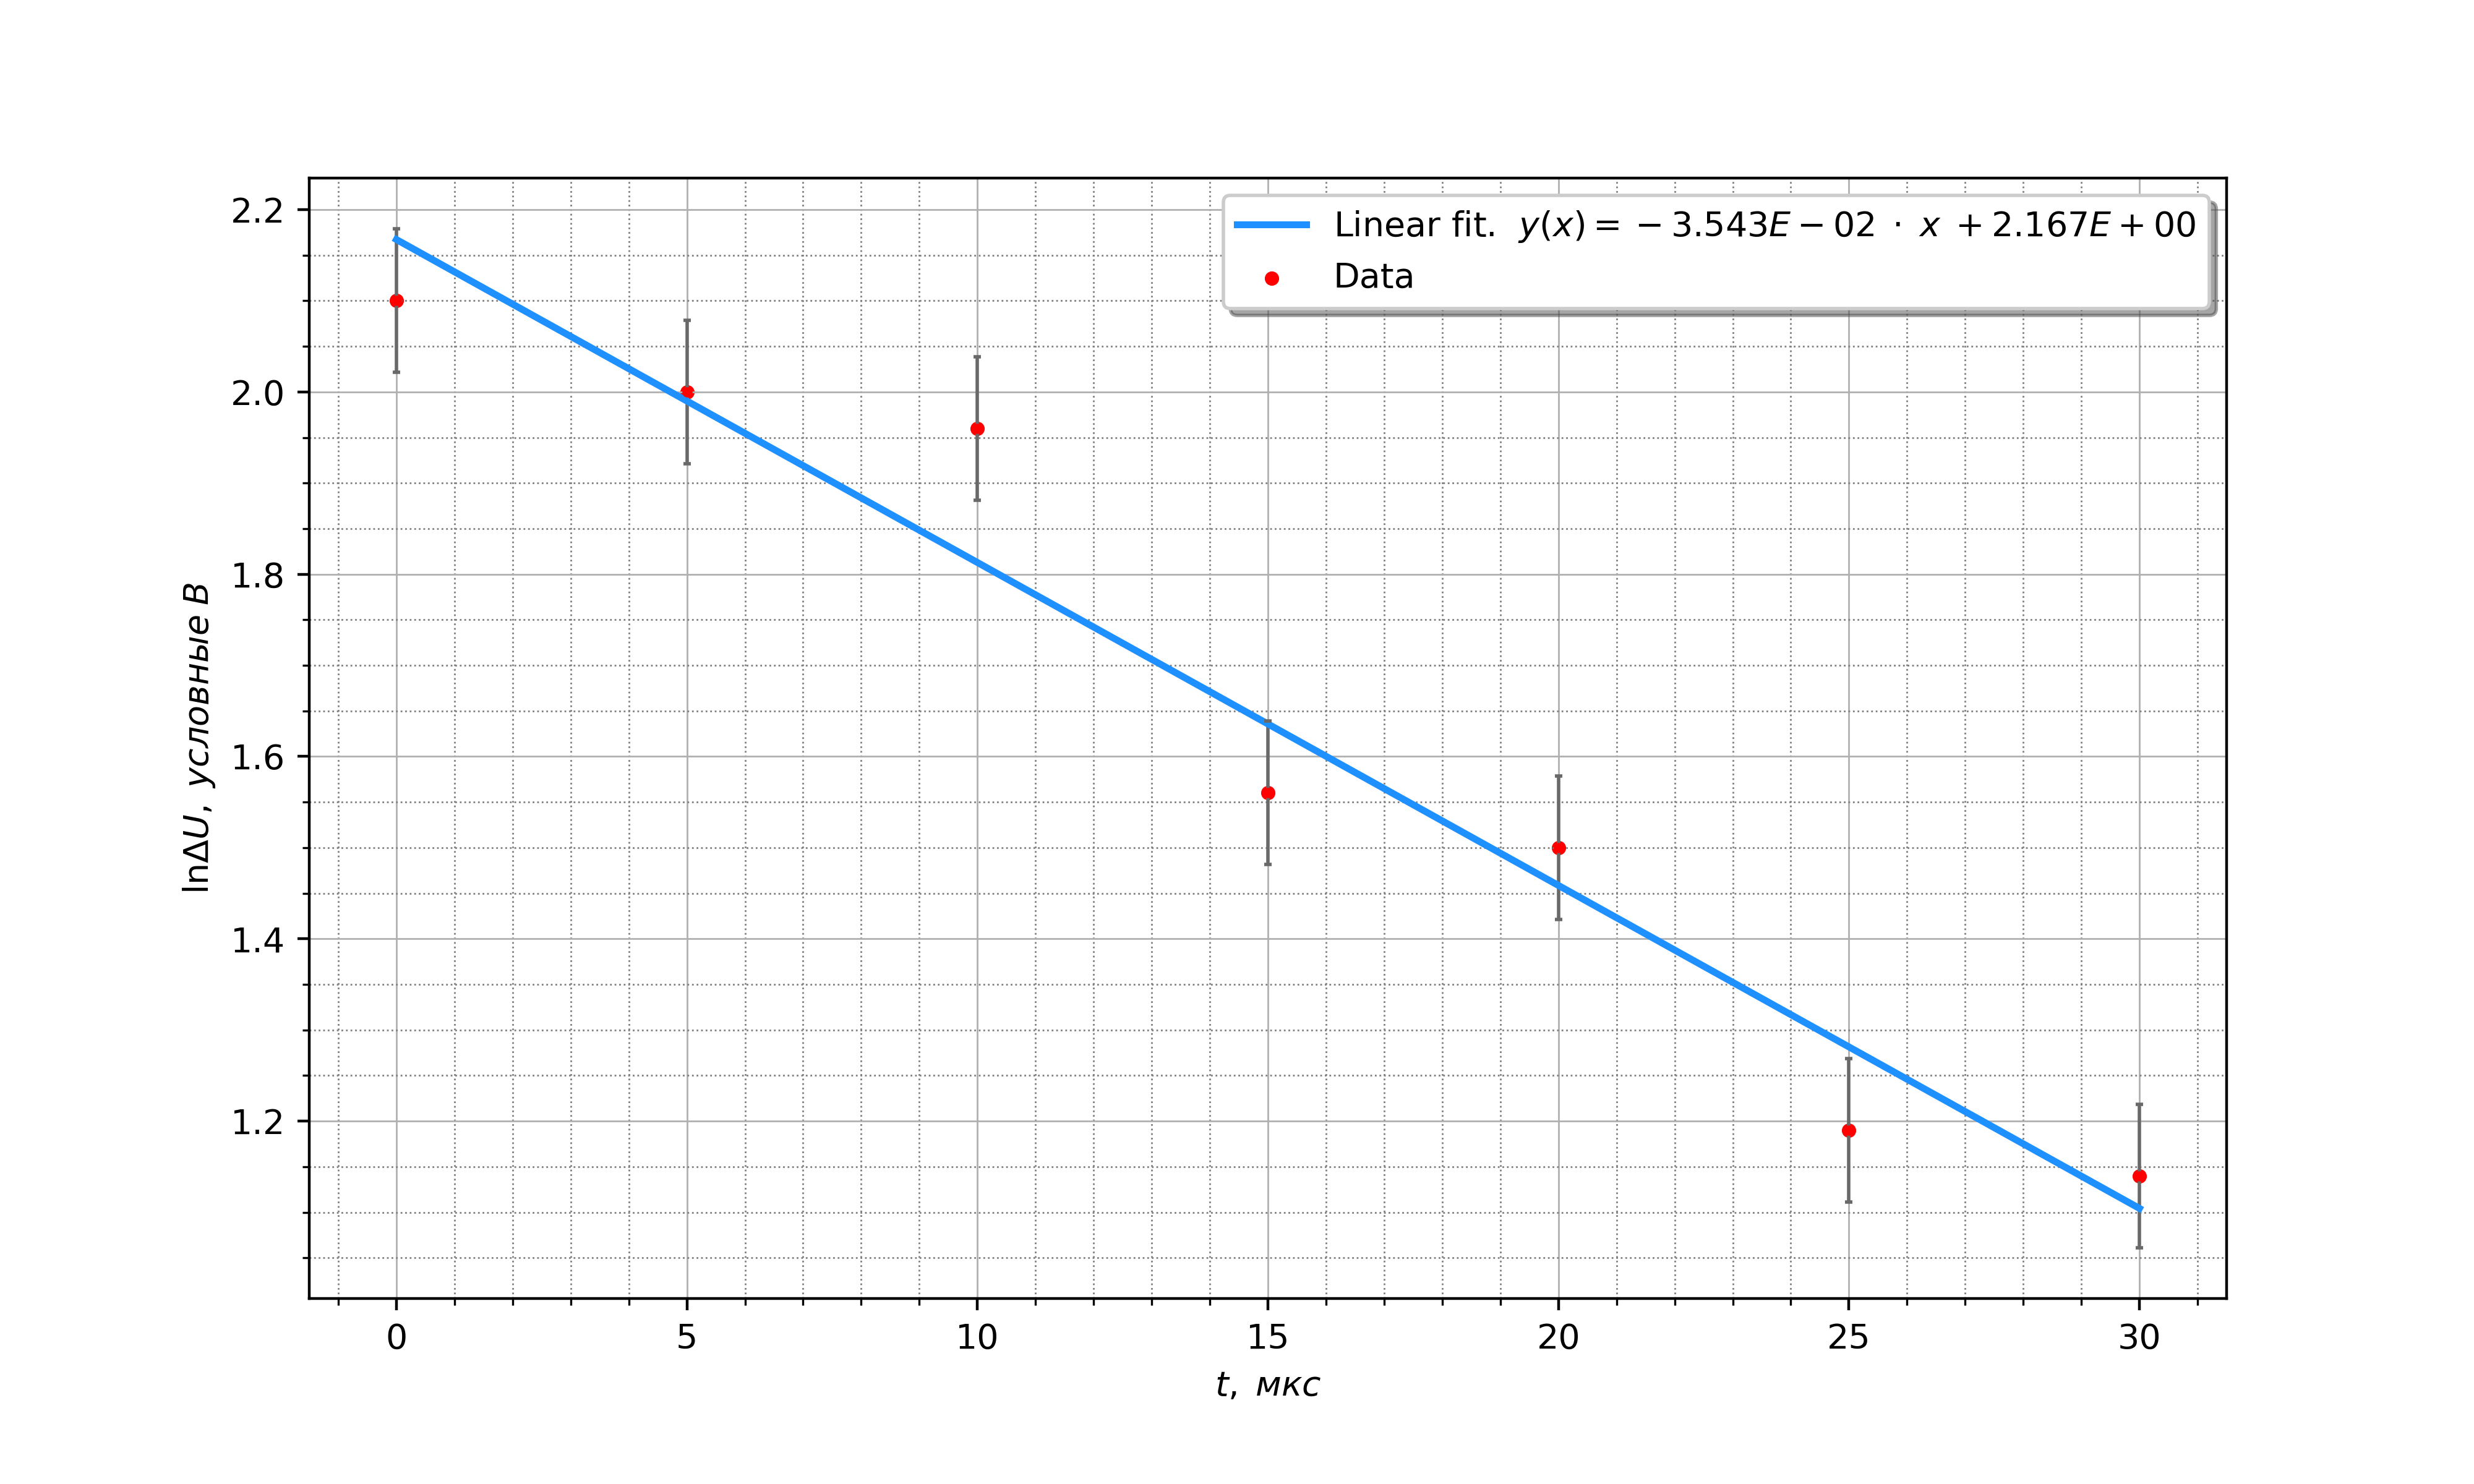
\includegraphics[scale = 0.7]{graph.png}
        \caption{}
        \label{}
    \end{center}
\end{figure}

Аппроксимируем набор данных в полулогорифмическом масштабе линейным уравнением уравнением $ln{\Delta U} = -\frac{t}{\tau} + \ln{C}$, из коэффициентов аппроксимации ($y(x) = a\cdot x + b$) $a = (3.54 \pm 0.35)\cdot 10^{-2}$, $b = 2.17 \pm 0.06$ определим 
время жизни электронов:

\begin{center}
    \fbox{$\tau = \frac{-1}{a} = 28.2 \pm 2.8\; мкс$}
\end{center}

	



\end{document}